\documentclass{article}

\usepackage{fancyhdr}
\usepackage{extramarks}
\usepackage{amsmath}
\usepackage{amsthm}
\usepackage{amsfonts}
\usepackage{tikz}
\usepackage[plain]{algorithm}
\usepackage{algpseudocode}
\usepackage{xcolor}
\usepackage{listings}
\usepackage{graphicx}
\usepackage{float}

\usetikzlibrary{automata,positioning}

%
% Basic Document Settings
%

\topmargin=-0.45in
\evensidemargin=0in
\oddsidemargin=0in
\textwidth=6.5in
\textheight=9.0in
\headsep=0.25in

\linespread{1.1}

\pagestyle{fancy}
\lhead{\hmwkAuthorName}
\chead{\hmwkClass\ (\hmwkClassInstructor\ \hmwkClassTime): \hmwkTitle}
\rhead{\firstxmark}
\lfoot{\lastxmark}
\cfoot{\thepage}

\renewcommand\headrulewidth{0.4pt}
\renewcommand\footrulewidth{0.4pt}

\setlength\parindent{0pt}

\lstdefinestyle{lfonts}{ 
    basicstyle = \footnotesize\ttfamily, 
    stringstyle = \color{purple}, 
    keywordstyle = \color{blue!60!black}\bfseries, 
    commentstyle = \color{olive}\scshape, 
} 
\lstdefinestyle{lnumbers}{ 
    numbers = left, 
    numberstyle = \tiny, 
    numbersep = 1em, 
    firstnumber = 1, 
    stepnumber = 1, 
} 
\lstdefinestyle{llayout}{ 
    breaklines = true, 
    tabsize = 2, 
    columns = flexible, 
} 
\lstdefinestyle{lgeometry}{ 
    xleftmargin = 20pt, 
    xrightmargin = 0pt, 
    frame = tb, 
    framesep = \fboxsep, 
    framexleftmargin = 20pt, 
} 
\lstdefinestyle{lgeneral}{ 
    style = lfonts, 
    style = lnumbers, 
    style = llayout, 
    style = lgeometry, 
} 
\lstdefinestyle{python}{ 
    language = {Python}, 
    style = lgeneral, 
}

%
% Create Problem Sections
%

\newcommand{\enterProblemHeader}[1]{
    \nobreak\extramarks{}{Problem \arabic{#1} continued on next page\ldots}\nobreak{}
    \nobreak\extramarks{Problem \arabic{#1}}{Problem \arabic{#1} continued on next page\ldots}\nobreak{}
}

\newcommand{\exitProblemHeader}[1]{
    \nobreak\extramarks{Problem \arabic{#1}}{Problem \arabic{#1} continued on next page\ldots}\nobreak{}
    \stepcounter{#1}
    \nobreak\extramarks{Problem \arabic{#1}}{}\nobreak{}
}

\setcounter{secnumdepth}{0}
\newcounter{partCounter}
\newcounter{homeworkProblemCounter}
\setcounter{homeworkProblemCounter}{1}
\nobreak\extramarks{Problem \arabic{homeworkProblemCounter}}{}\nobreak{}

%
% Homework Problem Environment
%
% This environment takes an optional argument. When given, it will adjust the
% problem counter. This is useful for when the problems given for your
% assignment aren't sequential. See the last 3 problems of this template for an
% example.
%
\newenvironment{homeworkProblem}[1][-1]{
    \ifnum#1>0
        \setcounter{homeworkProblemCounter}{#1}
    \fi
    \section{Problem \arabic{homeworkProblemCounter}}
    \setcounter{partCounter}{1}
    \enterProblemHeader{homeworkProblemCounter}
}{
    \exitProblemHeader{homeworkProblemCounter}
}

%
% Homework Details
%   - Title
%   - Due date
%   - Class
%   - Section/Time
%   - Instructor
%   - Author
%

\newcommand{\hmwkTitle}{Homework\ \#4}
\newcommand{\hmwkDueDate}{November 6, 2019}
\newcommand{\hmwkClass}{Advanced Computer Security}
\newcommand{\hmwkClassTime}{}
\newcommand{\hmwkClassInstructor}{Professor Jiageng Chen}
\newcommand{\hmwkAuthorName}{\textbf{Ruochen LIU}}

%
% Title Page
%

\title{
    \vspace{2in}
    \textmd{\textbf{\hmwkClass:\ \hmwkTitle}}\\
    \normalsize\vspace{0.1in}\small{Due\ on\ \hmwkDueDate\ at 9:00pm}\\
    \vspace{0.1in}\large{\textit{\hmwkClassInstructor\ \hmwkClassTime}}
    \vspace{3in}
}

\author{\hmwkAuthorName}
\date{}

\renewcommand{\part}[1]{\textbf{\large Part \Alph{partCounter}}\stepcounter{partCounter}\\}

%
% Various Helper Commands
%

% Useful for algorithms
\newcommand{\alg}[1]{\textsc{\bfseries \footnotesize #1}}

% For derivatives
\newcommand{\deriv}[1]{\frac{\mathrm{d}}{\mathrm{d}x} (#1)}

% For partial derivatives
\newcommand{\pderiv}[2]{\frac{\partial}{\partial #1} (#2)}

% Integral dx
\newcommand{\dx}{\mathrm{d}x}

% Alias for the Solution section header
\newcommand{\solution}{\textbf{\large Solution}}

% Probability commands: Expectation, Variance, Covariance, Bias
\newcommand{\E}{\mathrm{E}}
\newcommand{\Var}{\mathrm{Var}}
\newcommand{\Cov}{\mathrm{Cov}}
\newcommand{\Bias}{\mathrm{Bias}}

\begin{document}

\maketitle

\pagebreak

\begin{homeworkProblem}           

    \textbf{a):}
    First of all, we can get the differential table of two S-boxes by the given S-box, the code can be seen below, and so is the table:
\begin{lstlisting}[style = python]
def int2bin(num: int) -> str:
    return bin(int(num))[2:].zfill(8)


def oct_xor(s: int, t: int) -> str:
    return oct(int(oct(s), 8) ^ int(oct(t), 8))[2:]


s_box_1 = {
    "0": 0,
    "1": 5,
    "2": 3,
    "3": 2,
    "4": 6,
    "5": 1,
    "6": 4,
    "7": 7
}

differential_table_1 = []
tmp = []
for j in range(8):
    tmp.append(0)
for i in range(8):
    differential_table_1.append(tmp)

for xor_result in range(8):
    print('fixed xor result is: ', xor_result)
    for i in range(8):
        print('i = ', i)
        print('s[i] = ', s_box_1[str(i)])
        j = i ^ xor_result
        print('j = ', j)
        print('s[j] = ', s_box_1[str(j)])
        si_xor_sj = s_box_1[str(i)] ^ s_box_1[str(j)]
        print('====================')
        print(si_xor_sj)
        print('====================')
        differential_table_1[xor_result][int(si_xor_sj)] += 1
    print(differential_table_1)
    for m in range(8):
        for n in range(8):
            differential_table_1[m][n] = 0


s_box_2 = {
    "0": 0,
    "1": 5,
    "2": 10,
    "3": 11,
    "4": 20,
    "5": 17,
    "6": 22,
    "7": 23,
    "8": 9,
    "9": 12,
    "10": 3,
    "11": 2,
    "12": 13,
    "13": 8,
    "14": 15,
    "15": 14,
    "16": 18,
    "17": 21,
    "18": 24,
    "19": 27,
    "20": 6,
    "21": 1,
    "22": 4,
    "23": 7,
    "24": 26,
    "25": 29,
    "26": 16,
    "27": 19,
    "28": 30,
    "29": 25,
    "30": 28,
    "31": 31,
}

differential_table_2 = []
tmp = []
for j in range(32):
    tmp.append(0)
for i in range(32):
    differential_table_2.append(tmp)

for xor_result in range(32):
    # print('fixed xor result is: ', xor_result)
    for i in range(32):
        # print('i = ', i)
        # print('s[i] = ', s_box_2[str(i)])
        j = i ^ xor_result
        # print('j = ', j)
        # print('s[j] = ', s_box_2[str(j)])
        si_xor_sj = s_box_2[str(i)] ^ s_box_2[str(j)]
        # print('====================')
        # print(si_xor_sj)
        # print('====================')
        differential_table_2[xor_result][int(si_xor_sj)] += 1
    if xor_result == 31:
        print(differential_table_2[0])
    for m in range(32):
        for n in range(32):
            differential_table_2[m][n] = 0
\end{lstlisting}
And I put the result in a xlsx file, it looks like below:
\begin{figure}[H]
   	\centering
    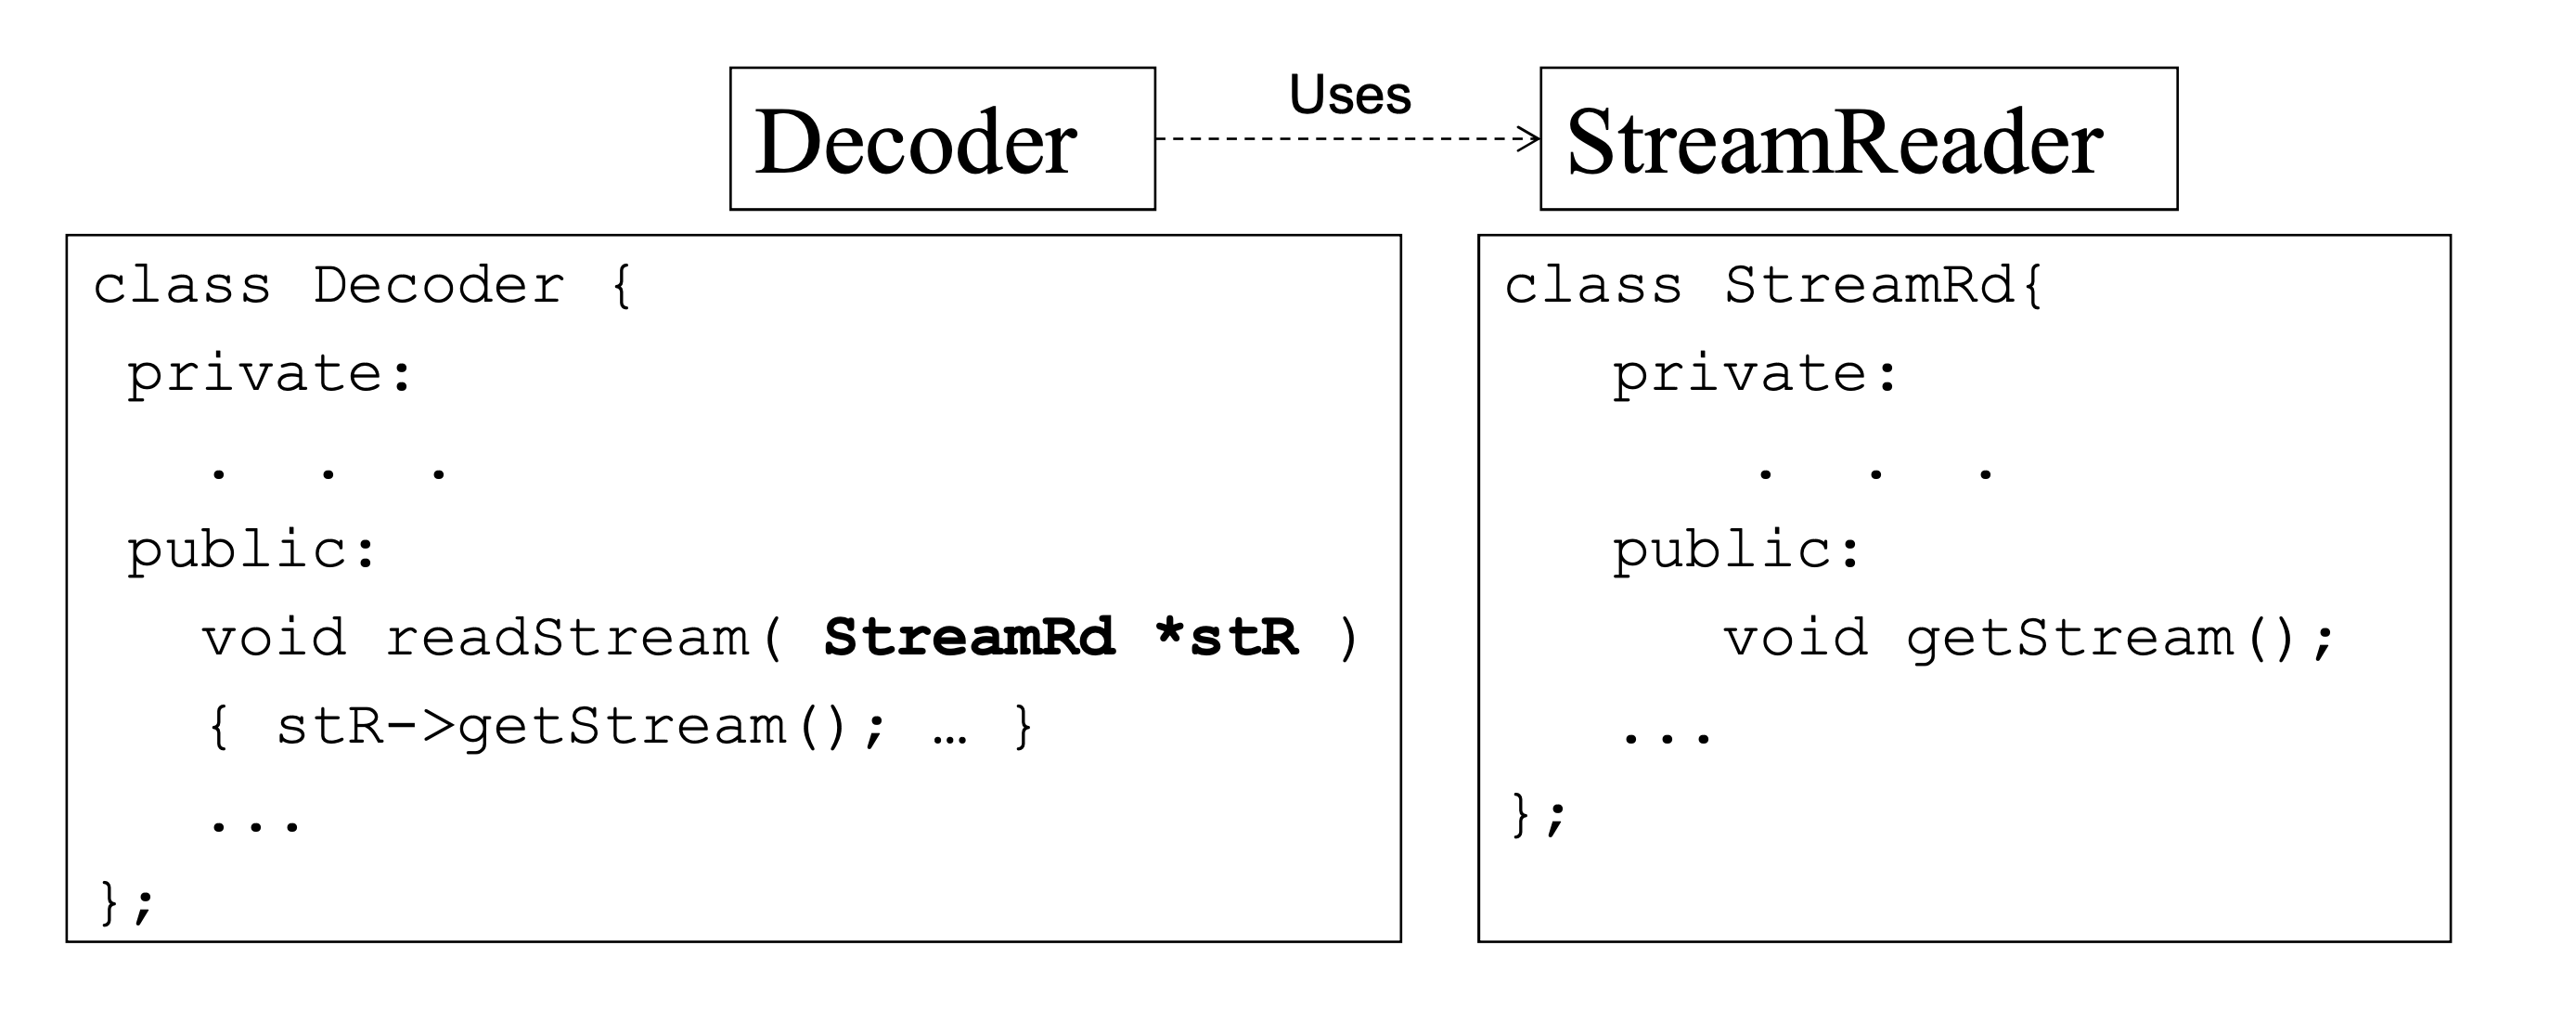
\includegraphics[width=15cm]{1.eps}
   	\caption{differential table for sbox 1}
    \label{fig-sample}
\end{figure}
And differential table for sbox 2:
\begin{figure}[H]
   	\centering
    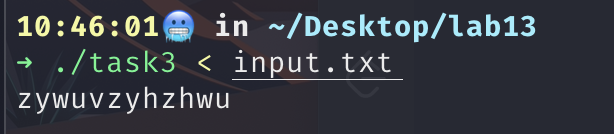
\includegraphics[width=16cm]{2.eps}
   	\caption{differential table for sbox 2}
    \label{fig-sample}
\end{figure}
\begin{figure}[H]
   	\centering
    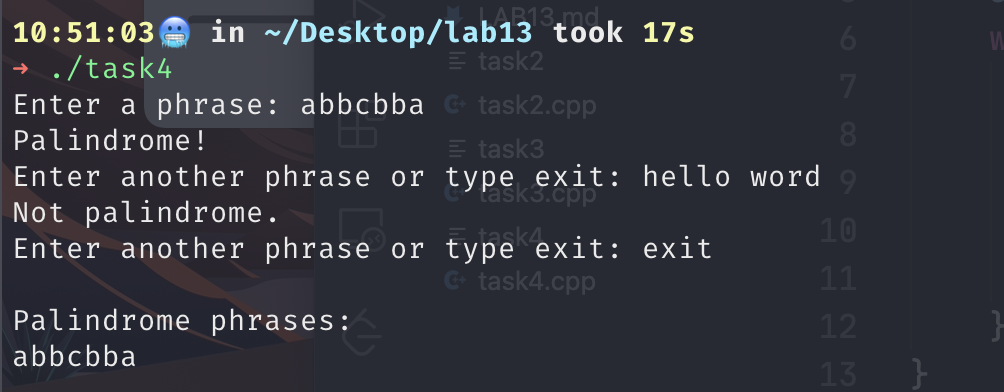
\includegraphics[width=16cm]{3.eps}
   	\caption{differential table for sbox 2}
    \label{fig-sample}
\end{figure}
After we get the differential table, in order to build an effective discriminator, we input more zeros as much as possible, and in order to get as few activation sboxes as possible, so that we can avoid many probability losses.
\\
We start with the input differential that $(0,0,0,0,0,0,0,0,0,0,0,0,0,0,0,0,1)$ as the left branch of input in raindrop, and the right branch is chosen for all zeros $(0,0,0,0,0,0,0,0,0,0,0,0,0,0,0,0)$, it is noted that in the left branch, we could reshape the input as a $4*4$ matrix in which elements at the first and the third row are 3-bits and others are 5-bits. It looks like below:
\begin{figure}[H]
   	\centering
    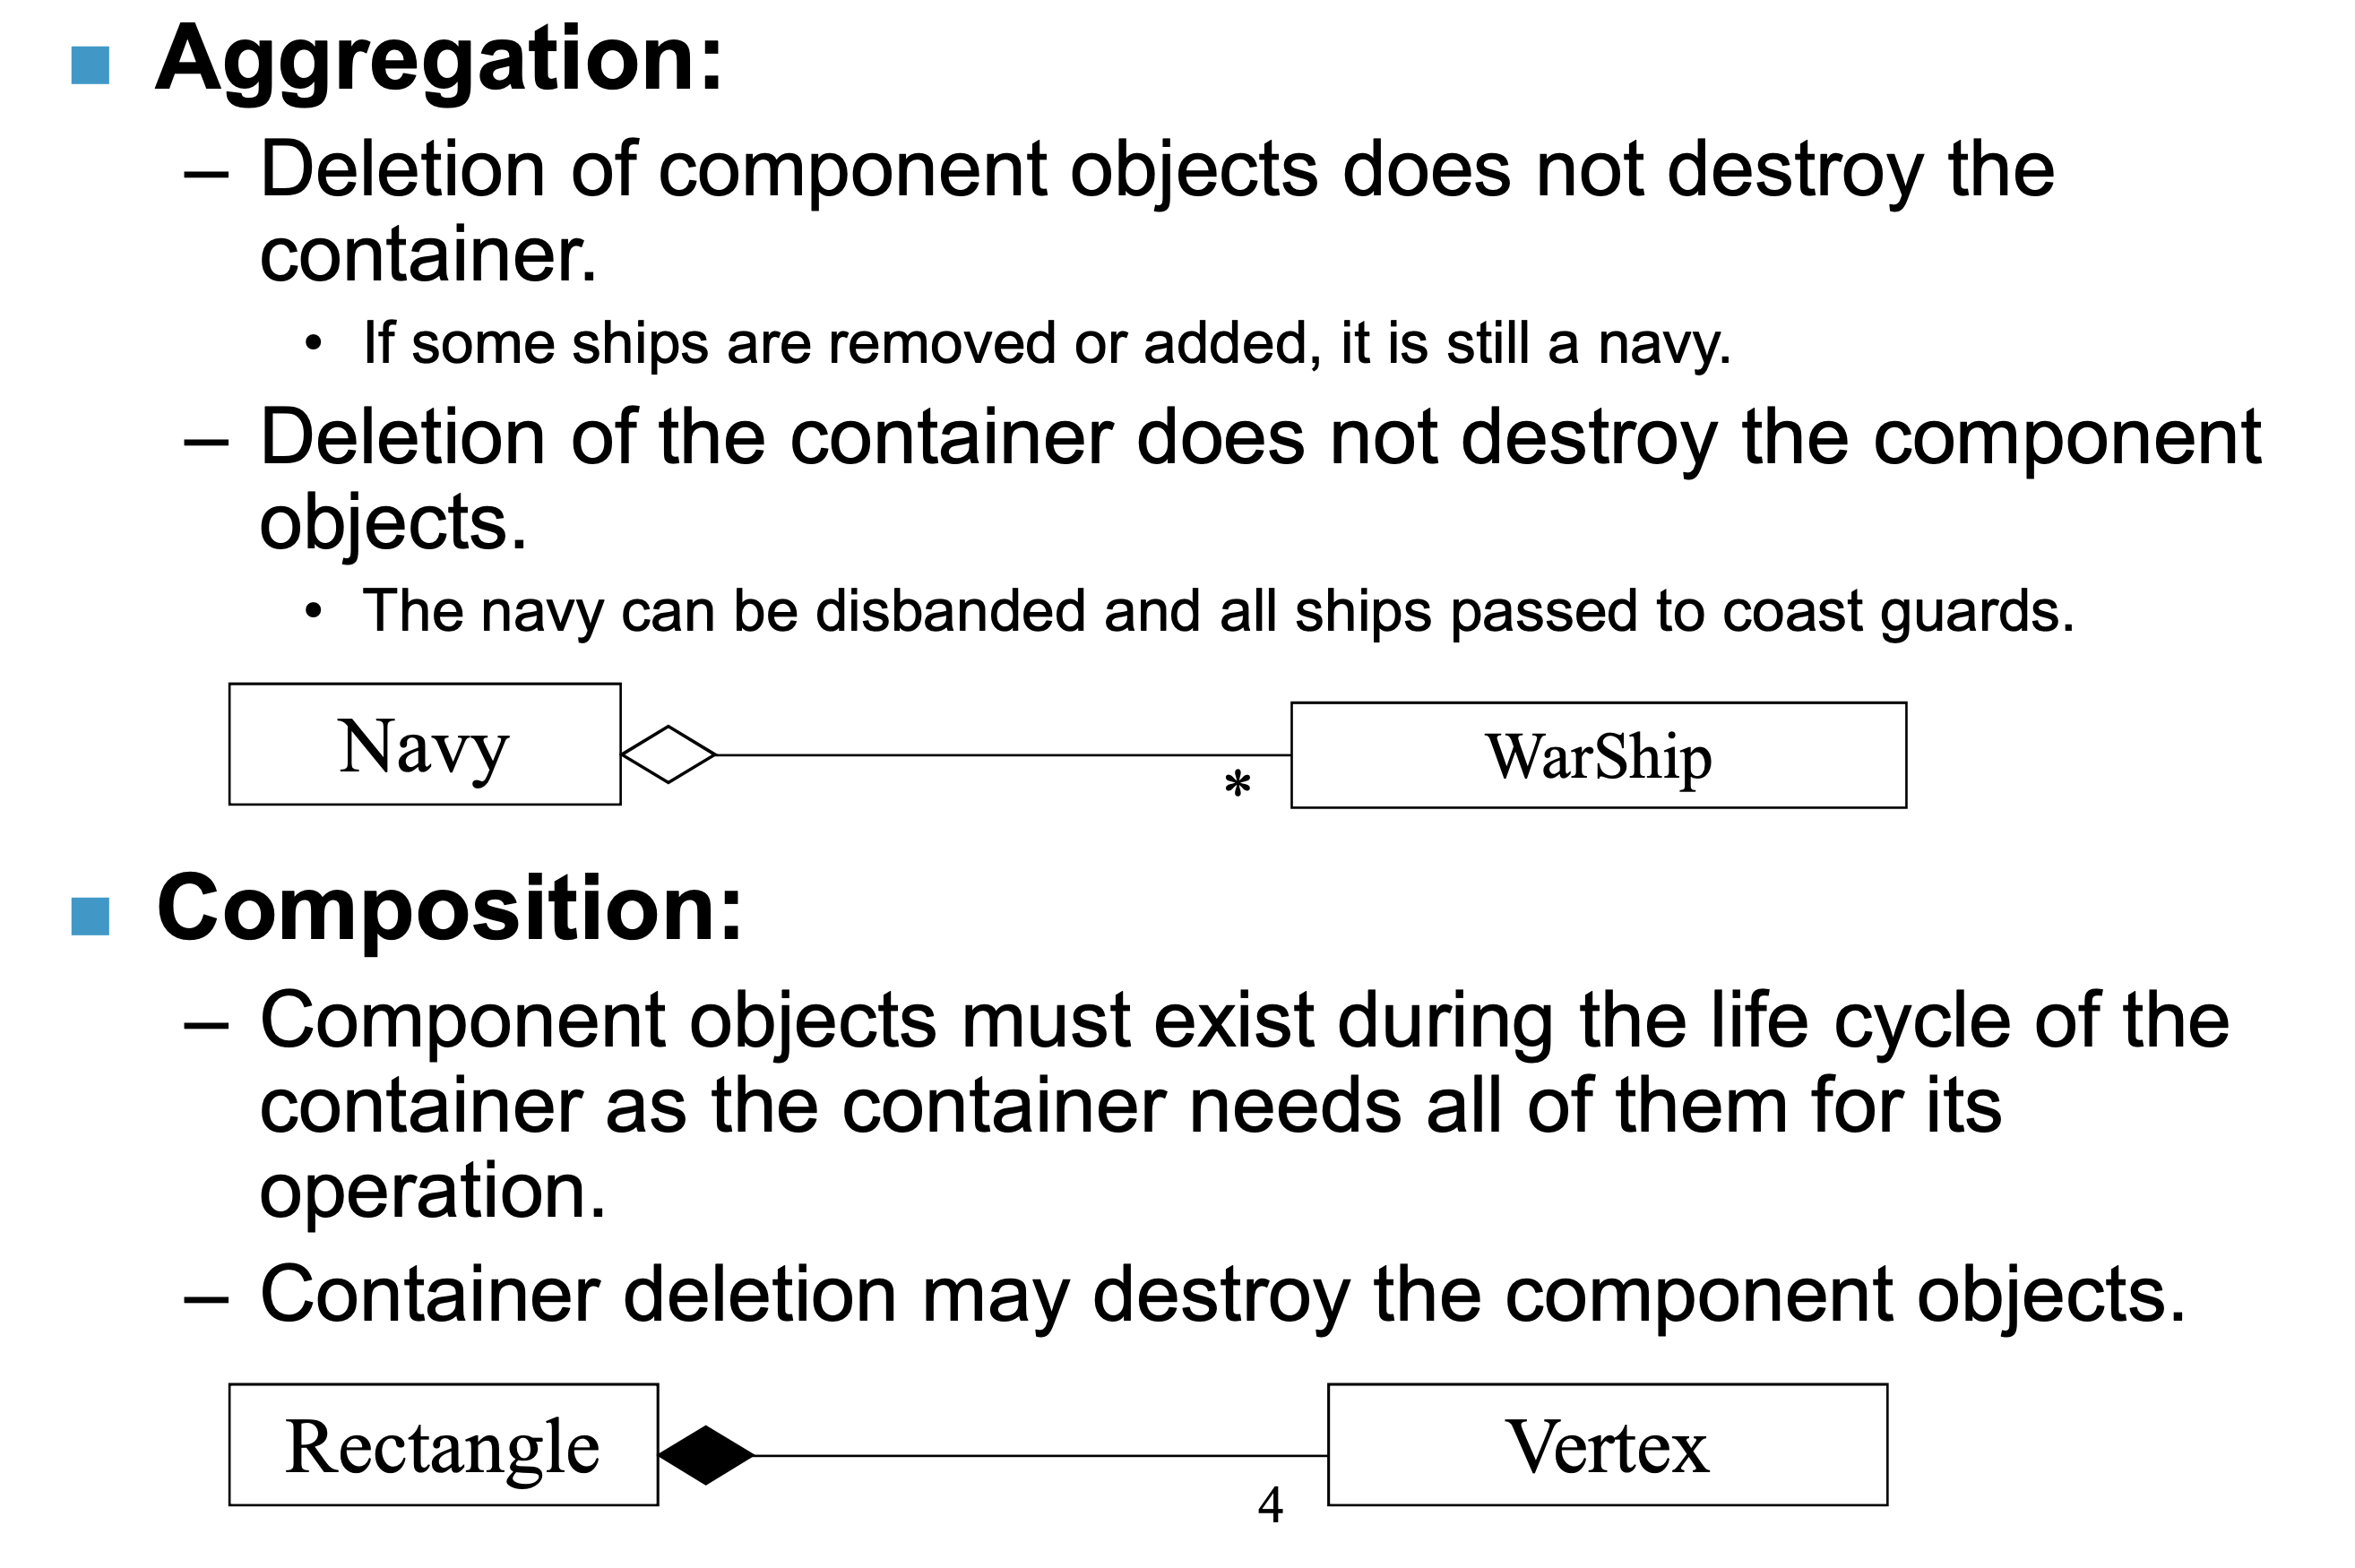
\includegraphics[width=4cm]{4.eps}
   	\caption{input shape of left}
    \label{fig-sample}
\end{figure}
In the matrix, $p_0,p_4,p_8,p_{12},p_2,p_6,p_{10},p_{14}$ are 3-bits and others are 5-bits.
\\
And it should be noted that the input is differential value of two plaintext, and we want to find a discriminative path to another differential value. So we input matrix, and search in differential table to chose a path with the biggest probability instead of computing output of sbox!
\\
\\
The main idea is that at first we fix a differential value, for example f. Then we travel all the pair of input which generate differential value is f. For each pair we compute the value of $S[m_0] \oplus S[m_1]$ and counter the number of each differential value appears. Sometimes we can found a value which is obviously appear more than others. So there is a path of high probability, it is what we called discriminator.
\\
For seeking this kind of effective differentiator, we take differential value as plaintext, and use differential table replace the sboxes. In each time we chose the path with the biggest probability of each differential table.
\\
For example, if we have a input of $[0, 0, 0, 0, 0, 0, 0, 0, 0, 0, 0, 0, 0, 0, 0, 1]$ for left branch and $[0, 0, 0, 0, 0, 0, 0, 0, 0, 0, 0, 0, 0, 0, 0, 0]$ for right branch. Because 1 is at the fourth row, so we search the differential table 2.
\begin{figure}[H]
   	\centering
    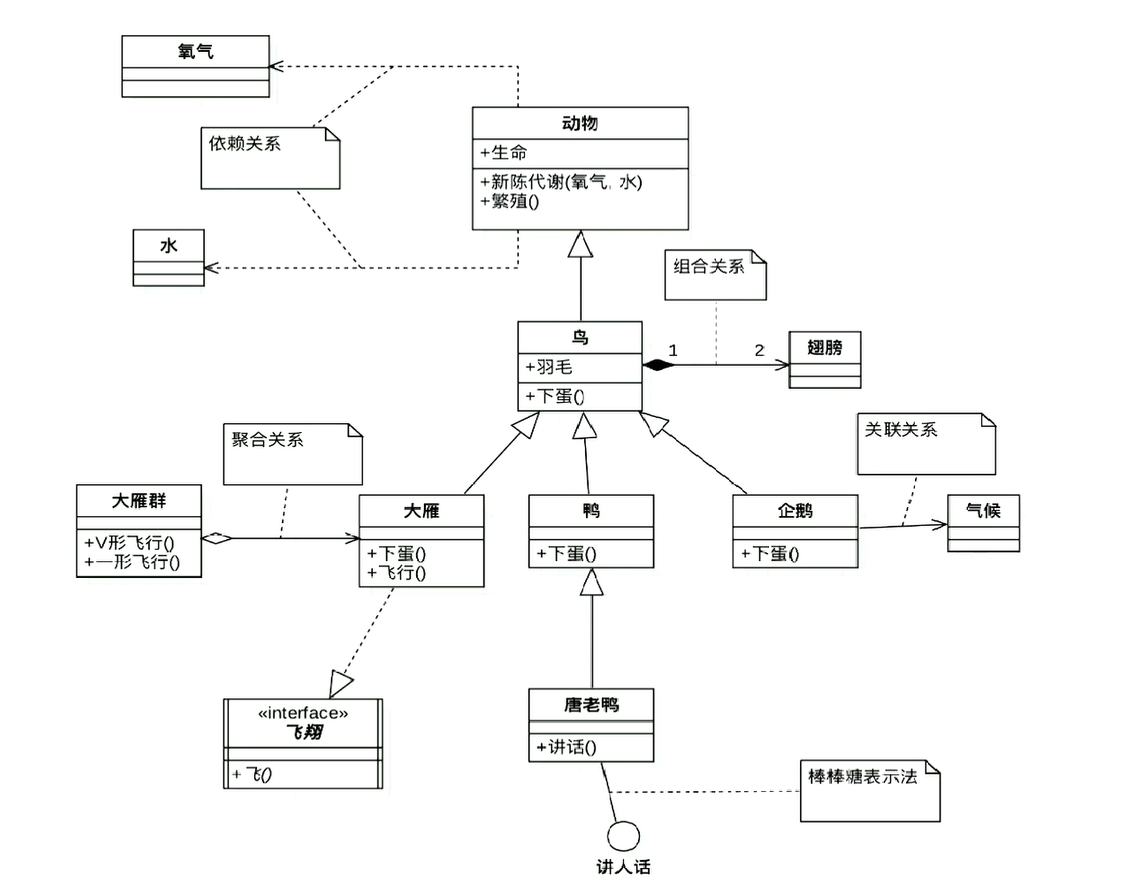
\includegraphics[width=15cm]{7.png}
   	\caption{differential table 2}
    \label{fig-sample}
\end{figure}
Notice that the path from differential 1 to 1 has the most frequency, so we chose the path $(1 \rightarrow 1)$, and now the input is $[0, 0, 0, 0, 0, 0, 0, 0, 0, 0, 0, 0, 0, 0, 0, 1]$.
\\
\\
The code is right below:
\begin{lstlisting}[style = python]
def choose_path(state: List[int], prob: float) -> dict:
    print('original state is ', state)
    new_state = []
    for index, i in enumerate(state):
        # print('i is ', i)
        max_path = -1
        max_p = -1
        if index < 4 or (7 < index < 12):
            for key in DT1[i]:
                if DT1[i][key] > max_p:
                    max_p = DT1[i][key]
                    max_path = key
            # print('prob. is ', max_p / 8)
            prob *= max_p / 8
        elif (3 < index < 8) or (11 < index < 16):
            for key in DT2[i]:
                if DT2[i][key] > max_p:
                    max_p = DT2[i][key]
                    max_path = key
            # print('prob. is ', max_p / 32)
            prob *= max_p / 32

        new_state.append(max_path)
    print('new state after choose path is ', new_state)
    print('the prob. of path is', str(prob), ', more than uniform?', str(prob > uniform_prob))
    return {'s': new_state, 'p': prob}
\end{lstlisting}
DT1 and DT2 are the sboxes.
\\
After that, we put the differential value into the raindrop, the structure is below:
\begin{figure}[H]
   	\centering
    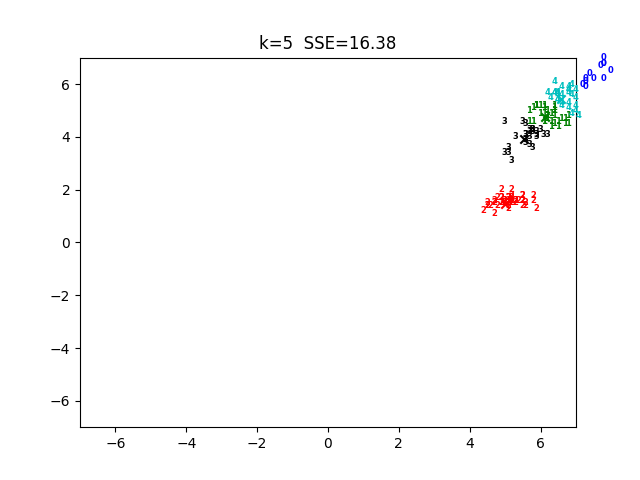
\includegraphics[width=10cm]{5.eps}
   	\caption{input shape of left}
    \label{fig-sample}
\end{figure}
In the round function, there are three steps. First is sbox function. Then mix row which makes input to multiple a mixer matrix. The last is bitwise rotate. The code can be seen below:
\begin{lstlisting}[style = python]
def mix_row(state: List[int]) -> List[int]:
    new_state = [0] * 16
    # row number 1
    new_state[0] = state[1] ^ state[3]
    new_state[1] = state[2] ^ state[3]
    new_state[2] = state[0]
    new_state[3] = state[0] ^ state[1]
    # row number 2
    new_state[4] = state[5] ^ state[7]
    new_state[5] = state[6] ^ state[7]
    new_state[6] = state[4]
    new_state[7] = state[4] ^ state[5]
    # row number 3
    new_state[8] = state[9] ^ state[11]
    new_state[9] = state[10] ^ state[11]
    new_state[10] = state[8]
    new_state[11] = state[8] ^ state[9]
    # row number 4
    new_state[12] = state[13] ^ state[15]
    new_state[13] = state[14] ^ state[15]
    new_state[14] = state[12]
    new_state[15] = state[12] ^ state[13]
    # print('new state after mix row is ', new_state)
    return new_state
\end{lstlisting}
This is mix row function.
\begin{lstlisting}[style = python]
def int2bin(num: int, pad: int) -> str:
    return bin(int(num))[2:].zfill(pad)


# int_value is number for shift
# k is number of shift bit
# bit is length of binary
def circular_shift_left(int_value: int, k: int, bit=16) -> str:
    k = k % bit
    bit_string = '{:0%db}' % bit
    bin_value = bit_string.format(int_value)  # 16 bit binary
    bin_value = bin_value[k:] + bin_value[:k]
    return bin_value


def bit_rot(state: List[int]) -> List[int]:
    new_state = [0] * 16
    new_state[0] = state[0]
    new_state[4] = state[4]
    new_state[8] = state[8]
    new_state[12] = state[12]
    for j in range(1, 4):
        # 2nd col is col1
        col = ''
        for i in range(4):
            index = j + 4 * i
            tmp = None
            if index < 4 or (7 < index < 12):
                # row 1 and 3 the length is 3
                tmp = int2bin(state[index], 3)
            elif (3 < index < 8) or (11 < index < 16):
                # row 2 and 4 the length is 5
                tmp = int2bin(state[index], 5)
            col += tmp
        new_col = circular_shift_left(int(col, 2), 6, 16)
        for i in range(4):
            index = j + 4 * i
            if index < 4 or (7 < index < 12):
                # row 1 and 3 the length is 3
                s = new_col[index - 1:index - 1 + 3]
                new_state[index] = int(s, 2)
            elif (3 < index < 8) or (11 < index < 16):
                # row 2 and 4 the length is 5
                s = new_col[index - 1:index - 1 + 5]
                new_state[index] = int(s, 2)

    # print('new state after bit row is ', new_state)
    return new_state
\end{lstlisting}
This is bitwise rotate, specifically, it is to connect the binary of the input, and bitwise shift left.
\\
Then the result of round function is used to xor with the result of right branch xor with round key. And the original left branch will be the next right branch and the next left branch is the result of xor operate mentioned before.
\\
Now consider the following equation:
\\
Assume we have a pair of plaintext and ciphertext named as $(m_0, c_0)$ and $(m_1,c_1)$, and $m_0$ can be divided as left part $m_{0l}$ and right part $m_{0r}$, so do the $c_0$.
\\
First we compute the differential value of $m_0$ and $m_1$:
\[
    \begin{split}
        m_0 \oplus m_1 &= m_{0l} \oplus m_{0r} || m_{1l} \oplus m_{1r}
    \end{split}
\]
Then is the differential value of $c_0$ and $c_1$:
\[
    \begin{split}
        c_0 &= c_{0l} || c_{0r}
        \\
        c_{0l} &= S[m_{0l}] \oplus m_{0r} \oplus kr
        \\
        c_{0r} &= m_{0l}
        \\
        c_0 \oplus c_1 &= c_{0l} \oplus c_{1l} || c_{0r} \oplus c_{1r}
        \\
        &= S[m_{0l}] \oplus m_{0r} \oplus kr \oplus S[m_{1l}] \oplus m_{1r} \oplus kr || m_{0l} \oplus m_{1l}
        \\
        &= S[m_{0l}] \oplus S[m_{1l}] \oplus m_{0r} \oplus m_{1r} || m_{0l} \oplus m_{1l}
    \end{split}
\]
From the equation above we can see that in each round, the output left is $S[m_{0l}] \oplus S[m_{1l}] \oplus m_{0r} \oplus m_{1r}$, but in our differential table, we compute the frequency of the path: $m_{0l} \oplus m_{1l}$ to $S[m_{0l}] \oplus S[m_{1l}]$.
\\
Thus, to remove $m_{0r} \oplus m_{1r}$, we need to make the result xor with the right branch of input, because the right branch of input is the differential value of $m_{0r}$ and $m_{1r}$, so the code is right below:
\begin{lstlisting}[style = python]
    print('the', str(m + 1), 'round...')
    ori_left_round_res = left_round_res[:]
    tmp = choose_path(left_round_res, init_prob)
    left_round_res = bit_rot(mix_row(tmp['s']))
    init_prob = tmp['p']

    right_str = ''
    for n in right_round_res:
        right_str += int2bin(n, 4)
    right_int = int(right_str, 2)

    r_kr = int(right_str, 2) ^ int(round_key[m], 2)

    left_str = ''
    for n in left_round_res:
        left_str += int2bin(n, 4)
    left_int = int(left_str, 2)

    new_left_int = left_int ^ r_kr ^ right_int
\end{lstlisting}
After that, we can get the output which is $[0, 0, 0, 2, 0, 0, 1, 16, 0, 0, 4, 2, 0, 4, 3, 16]$ for the example above. Next we start the new round, and it is the process.
\\
So we make a trial, to compute the cumulative probability per round, and the result is like below:
\begin{figure}[H]
   	\centering
    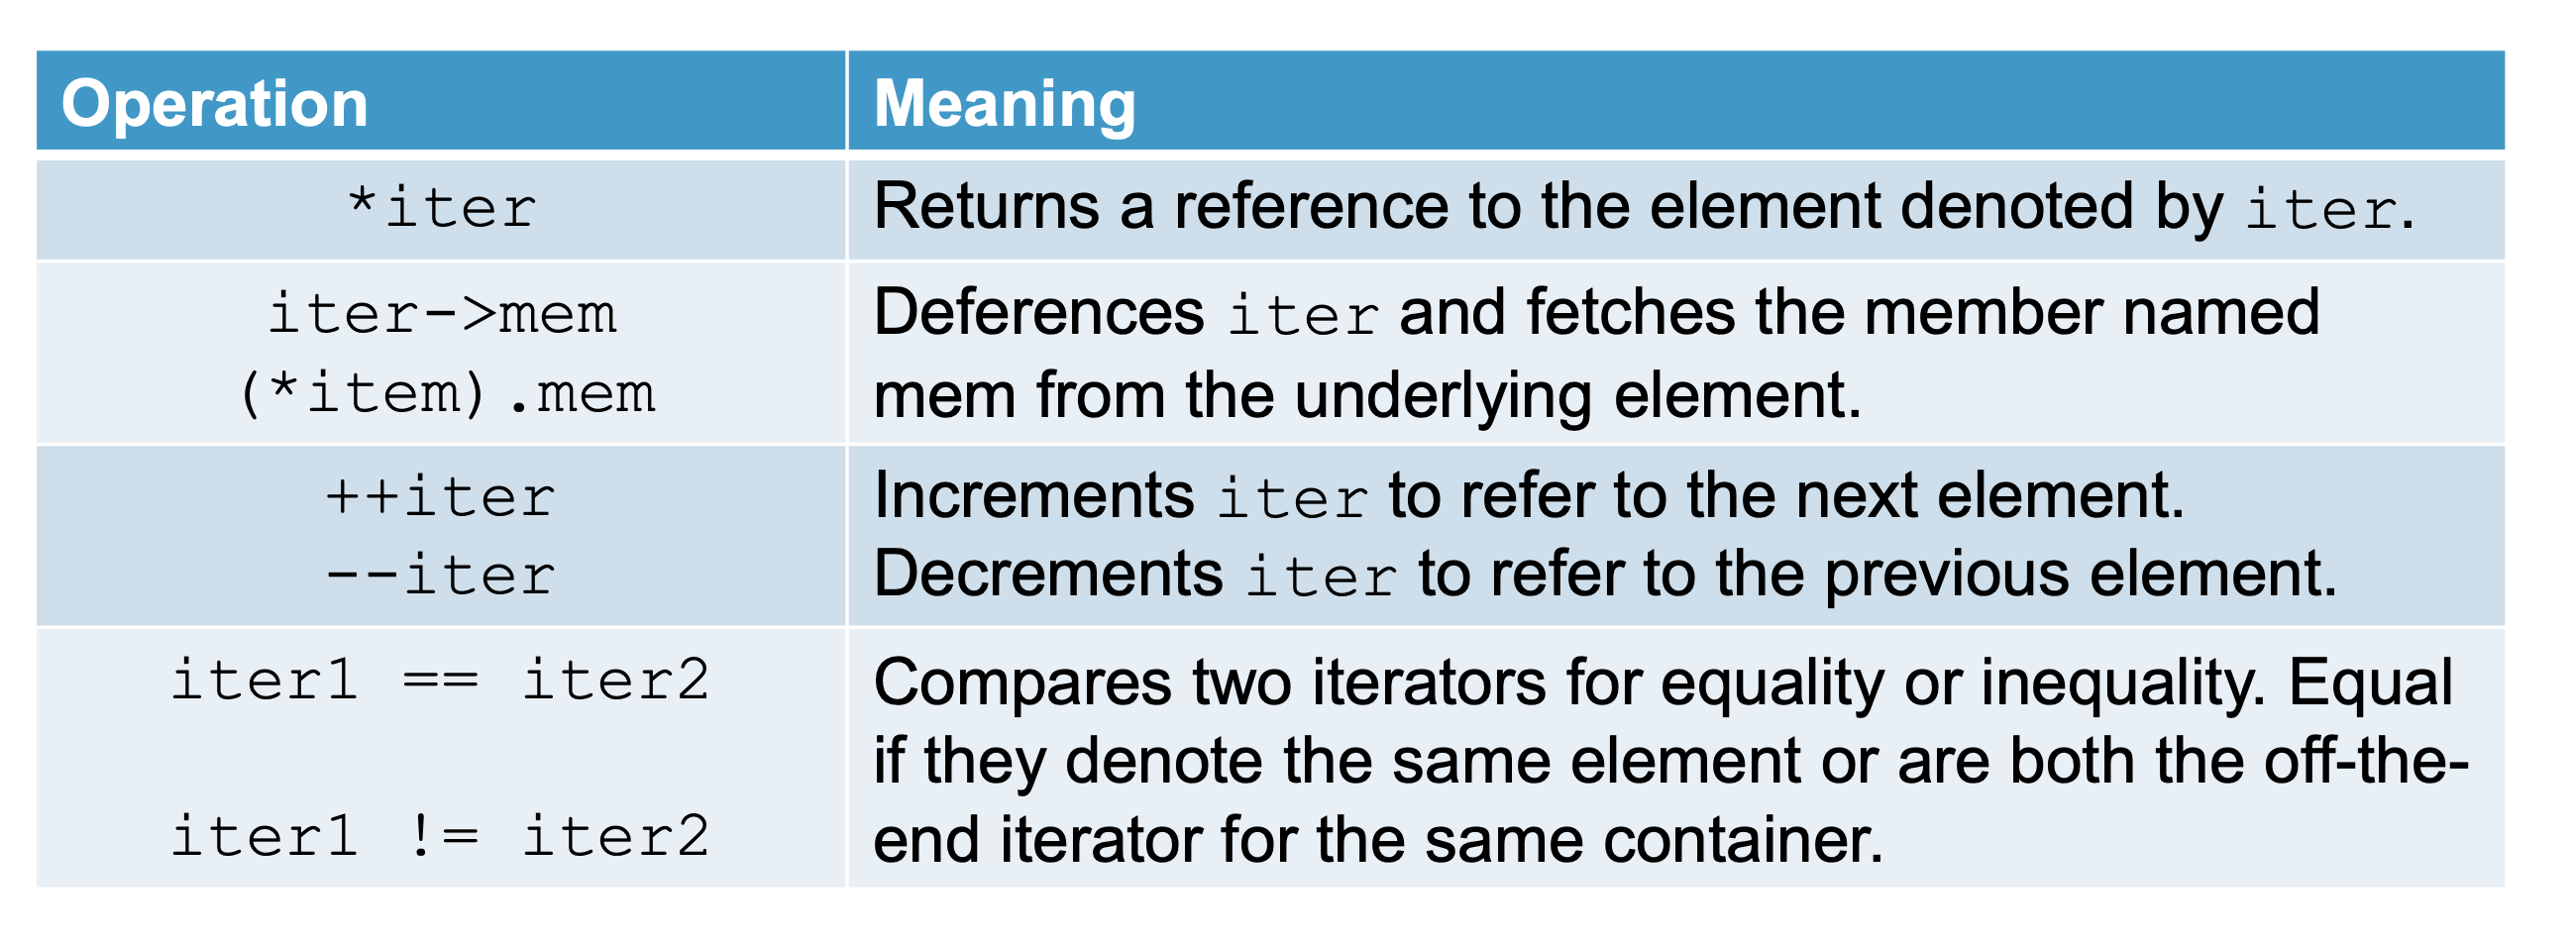
\includegraphics[width=16cm]{6.eps}
   	\caption{input shape of left}
    \label{fig-sample}
\end{figure}
In this trail, we can see the probability is less than $\frac{1}{2^{128}}$ in the last round, round six.
\\
So it is a valid discriminator of round five.
\\
The complete code can be seen below:
\begin{lstlisting}[style = python]
from typing import List

left = [0, 0, 0, 0, 0, 0, 0, 0, 0, 0, 0, 0, 0, 0, 0, 1]
right = [0, 0, 0, 0, 0, 0, 0, 0, 0, 0, 0, 0, 0, 0, 0, 0]
round_number = 6

uniform_prob = pow(1 / 2, 128)
init_prob = 1


def choose_path(state: List[int], prob: float) -> dict:
    print('original state is ', state)
    new_state = []
    for index, i in enumerate(state):
        # print('i is ', i)
        max_path = -1
        max_p = -1
        if index < 4 or (7 < index < 12):
            for key in DT1[i]:
                if DT1[i][key] > max_p:
                    max_p = DT1[i][key]
                    max_path = key
            # print('prob. is ', max_p / 8)
            prob *= max_p / 8
        elif (3 < index < 8) or (11 < index < 16):
            for key in DT2[i]:
                if DT2[i][key] > max_p:
                    max_p = DT2[i][key]
                    max_path = key
            # print('prob. is ', max_p / 32)
            prob *= max_p / 32

        new_state.append(max_path)
    print('new state after choose path is ', new_state)
    print('the prob. of path is', str(prob), ', more than uniform?', str(prob > uniform_prob))
    return {'s': new_state, 'p': prob}


def mix_row(state: List[int]) -> List[int]:
    new_state = [0] * 16
    # row number 1
    new_state[0] = state[1] ^ state[3]
    new_state[1] = state[2] ^ state[3]
    new_state[2] = state[0]
    new_state[3] = state[0] ^ state[1]
    # row number 2
    new_state[4] = state[5] ^ state[7]
    new_state[5] = state[6] ^ state[7]
    new_state[6] = state[4]
    new_state[7] = state[4] ^ state[5]
    # row number 3
    new_state[8] = state[9] ^ state[11]
    new_state[9] = state[10] ^ state[11]
    new_state[10] = state[8]
    new_state[11] = state[8] ^ state[9]
    # row number 4
    new_state[12] = state[13] ^ state[15]
    new_state[13] = state[14] ^ state[15]
    new_state[14] = state[12]
    new_state[15] = state[12] ^ state[13]
    # print('new state after mix row is ', new_state)
    return new_state


def int2bin(num: int, pad: int) -> str:
    return bin(int(num))[2:].zfill(pad)


# int_value is number for shift
# k is number of shift bit
# bit is length of binary
def circular_shift_left(int_value: int, k: int, bit=16) -> str:
    k = k % bit
    bit_string = '{:0%db}' % bit
    bin_value = bit_string.format(int_value)  # 16 bit binary
    bin_value = bin_value[k:] + bin_value[:k]
    return bin_value


def bit_rot(state: List[int]) -> List[int]:
    new_state = [0] * 16
    new_state[0] = state[0]
    new_state[4] = state[4]
    new_state[8] = state[8]
    new_state[12] = state[12]
    for j in range(1, 4):
        # 2nd col is col1
        col = ''
        for i in range(4):
            index = j + 4 * i
            tmp = None
            if index < 4 or (7 < index < 12):
                # row 1 and 3 the length is 3
                tmp = int2bin(state[index], 3)
            elif (3 < index < 8) or (11 < index < 16):
                # row 2 and 4 the length is 5
                tmp = int2bin(state[index], 5)
            col += tmp
        new_col = circular_shift_left(int(col, 2), 6, 16)
        for i in range(4):
            index = j + 4 * i
            if index < 4 or (7 < index < 12):
                # row 1 and 3 the length is 3
                s = new_col[index - 1:index - 1 + 3]
                new_state[index] = int(s, 2)
            elif (3 < index < 8) or (11 < index < 16):
                # row 2 and 4 the length is 5
                s = new_col[index - 1:index - 1 + 5]
                new_state[index] = int(s, 2)

    # print('new state after bit row is ', new_state)
    return new_state


# key is a list which length is 8
def A(key: List[int]) -> List[int]:
    in_0 = key[0]
    in_1 = key[1]
    in_2 = key[2]
    in_3 = key[3]
    in_4 = key[4]
    in_5 = key[5]
    in_6 = key[6]
    in_7 = key[7]

    tmp_0 = (in_0 >> 10) ^ in_7
    tmp_1 = in_0
    tmp_2 = in_1
    tmp_3 = in_2
    tmp_4 = in_3
    tmp_5 = in_4
    tmp_6 = (in_2 >> 15) ^ in_5
    tmp_7 = (in_1 >> 15) ^ in_6

    bin_str = int2bin(tmp_0, 16) + int2bin(tmp_1, 16) + int2bin(tmp_2, 16) + int2bin(tmp_3, 16) + int2bin(tmp_4,
                                                                                                          16) + int2bin(
        tmp_5, 16) + int2bin(tmp_6, 16) + int2bin(tmp_7, 16)

    output_str = circular_shift_left(int(bin_str, 2), 5, 128)

    r = [0] * 8
    for index in range(8):
        r[index] = int(output_str[index * 16:index * 16 + 16], 2)
    return r


# generate round key
tk_0 = [1, 2, 3, 4, 5, 6, 7, 8]
round_key = [''] * round_number
for i in range(round_number):
    tk_str = ''
    for j in tk_0:
        tk_str += int2bin(j, 16)
    tk_int = int(tk_str, 2)
    round_const = int(int2bin(round_number, 64) + '0000000000000000000000000000000000000000000000000000000000000000', 2)

    out_str = int2bin(tk_int ^ round_const, 128)

    result = [0] * 8
    for idx in range(8):
        result[idx] = int(out_str[idx * 16:idx * 16 + 16], 2)

    init_input = result
    for k in range(4):
        init_input = A(init_input)

    res = ''
    for l in init_input:
        res += int2bin(l, 16)
    round_key[i] = res[64:]

    tk_0 = init_input

left_round_res = left
right_round_res = right
for m in range(round_number):
    print('the', str(m + 1), 'round...')
    ori_left_round_res = left_round_res[:]
    tmp = choose_path(left_round_res, init_prob)
    left_round_res = bit_rot(mix_row(tmp['s']))
    init_prob = tmp['p']

    right_str = ''
    for n in right_round_res:
        right_str += int2bin(n, 4)
    right_int = int(right_str, 2)

    r_kr = int(right_str, 2) ^ int(round_key[m], 2)

    left_str = ''
    for n in left_round_res:
        left_str += int2bin(n, 4)
    left_int = int(left_str, 2)

    new_left_int = left_int ^ r_kr ^ right_int
    # new_left_int = left_int ^ r_kr
    new_left_str = int2bin(new_left_int, 64)
    # update left
    for index in range(16):
        if index < 4:
            # row 1 the length is 3
            left_round_res[index] = int(new_left_str[index * 3:index * 3 + 3], 2)
        elif 3 < index < 8:
            # row 2 the length is 5
            left_round_res[index] = int(new_left_str[12 + (index - 4) * 5: 12 + (index - 4) * 5 + 5], 2)
        elif 7 < index < 12:
            left_round_res[index] = int(new_left_str[32 + (index - 8) * 3:32 + (index - 8) * 3 + 3], 2)
        elif 11 < index < 16:
            left_round_res[index] = int(new_left_str[44 + (index - 12) * 5:44 + (index - 12) * 5 + 5], 2)
    print('state after round function is', left_round_res)
    # update right
    right_round_res = ori_left_round_res
\end{lstlisting}
\end{homeworkProblem}

\pagebreak

\end{document}
